\section{Related Work}
\label{sec:related}

\paragraph{Recursive model improvement.}
\begin{wrapfigure}{r}{0.55\textwidth}
\vspace{-10pt}
\centering
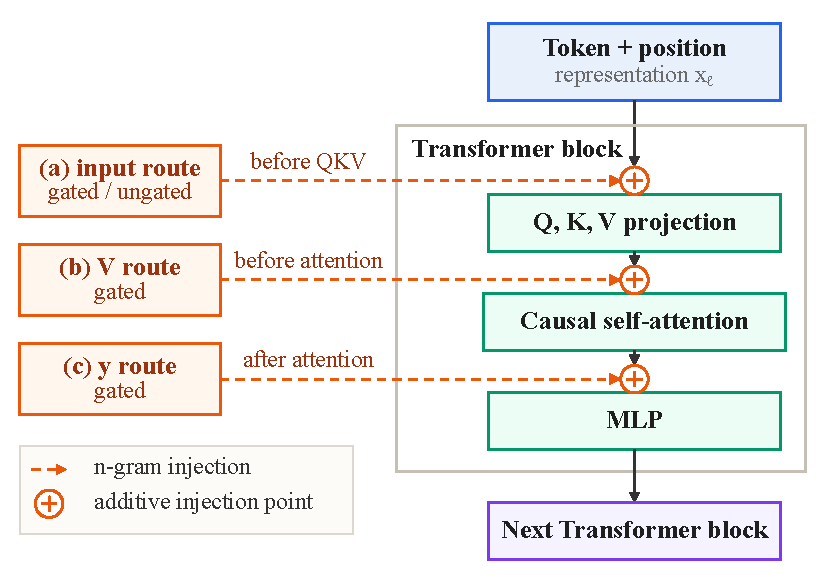
\includegraphics[width=0.55\textwidth]{figures/fig_transformer_ngram_injection_routes.pdf}
\caption{Three $n$-gram injection routes.}
\label{fig:injection-routes}
\vspace{-12pt}
\end{wrapfigure}
NanoGPT provides a compact implementation for training GPT-style language models \citep{karpathy2022nanogpt}. The autoresearch workflow places a language-model agent in a repeated cycle of modifying a trainer, running a budgeted experiment, and evaluating validation BPB \citep{karpathy2026autoresearch}. Related automated-research reports explore how agents can use earlier experiments to propose and combine improvements to language-model training \citep{recursive2026research}. Our work begins within this kind of search, but focuses on an unexpected training phenomenon and the conditions under which an automatically selected modification fails to generalize.

\paragraph{Over-encoding.}
Over-encoding augments token representations with embeddings of local token combinations. Figure~\ref{fig:injection-routes} distinguishes injection into the input representations, attention values ($v$), and attention output ($y$). Under this classification, N-Grammer's default placement is input-side: it combines latent bigram embeddings with token embeddings before the Transformer \citep{roy2022ngrammer}. The Over-Tokenized Transformer also uses input injection, adding projected multi-order $n$-gram embeddings while keeping the output vocabulary separate \citep{huang2025over}. SCONE follows the input-side route with contextualized embeddings for frequent $n$-grams, computed by an auxiliary model and cached for inference \citep{yu2025scone}. Engram extends this idea to multiple layers, adding gated $n$-gram memory to the residual stream before attention, which corresponds to multi-layer input injection in our terminology \citep{cheng2026engram}.Over-encoding also appears in record-setting recipes for Parameter Golf and the NanoGPT speedrun, where hash-indexed bigram embeddings augment input representations or layer inputs \citep{openai2026parametergolf,shah2026bigramgolf,modded_nanogpt_2024}. At production scale, the open-weight DeepSeek-V4.1-Flash incorporates Engram conditional memory, bringing this approach to a model with 552B backbone parameters and 196B memory parameters \citep{deepseek2026v41flash}. These studies demonstrate that over-encoding improves language-model efficiency and performance by expanding access to local context through sparse lookup, while our work identifies its risk of amplifying overfitting when finite training data are replayed.

\paragraph{Training with repeated data.}
Data-constrained scaling studies show that repeated tokens can remain useful, while their marginal value decreases as repetition increases \citep{muennighoff2023scaling}. \citet{hernandez2022repeated} study how repeated subsets affect language-model learning, including increases in test loss during training and changes in copying-related behavior. These results establish that replay can alter both generalization and internal computation. Forking adds a component-specific case: rapid, replay-aligned divergence associated with local n-gram memory, together with interventions that test the role of context frequency and memory access.

\paragraph{Good--Turing estimation.}
Good--Turing estimation uses frequency-of-frequencies statistics to estimate the probability mass of outcomes absent from a finite sample \citep{good1953population,gale1995good}. Its missing-mass estimate is the fraction of observations belonging to outcomes seen exactly once. Applied conditionally to an observed context, this estimates the probability assigned to continuations not represented in its training occurrences. This provides a statistical basis for studying incomplete continuation coverage. Relating that missing mass to a model's loss gap requires additional assumptions about how training changes predictions for seen and unseen continuations.